\mode*

% Since this a solution template for a generic talk, very little can
% be said about how it should be structured. However, the talk length
% of between 15min and 45min and the theme suggest that you stick to
% the following rules:  

% - Exactly two or three sections (other than the summary).
% - At *most* three subsections per section.
% - Talk about 30s to 2min per frame. So there should be between about
%   15 and 30 frames, all told.


\section{More counter-intuitive things}

\subsection{Secure multi-party computation}

\begin{frame}
  \begin{example}[Yao's Millionaires' Problem]
    \begin{itemize}
      \item Two millionaires meet in the street.
      \item They want to find out who is the richer.

        \pause{}

      \item However, they don't want to reveal how many millions they each 
        have.
    \end{itemize}
  \end{example}
\end{frame}

\begin{frame}
  \begin{idea}
    \begin{itemize}
      \uncover<1>{%
      \item We have \(n\) participants \(P_1, \ldots, P_n\).
      }
      \uncover<2>{%
      \item Each person has a \emph{secret} input value \(x_j\) for \(1\leq 
          j\leq n\).
      }
      \uncover<3>{%
      \item But they desperately want to know \(y = f(x_1, \ldots, x_n)\).
      }
    \end{itemize}
  \end{idea}
%\end{frame}
%\begin{frame}
  \begin{figure}
    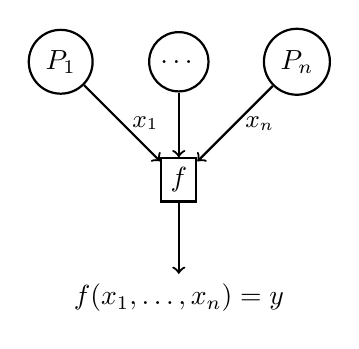
\begin{tikzpicture}[->,auto,node distance=1.5cm,
      thick,input node/.style={circle,draw},
      func node/.style={rectangle,draw}]

      \uncover<1,2,4>{%
      \node[input node] (1) {$P_1$};
      \node[input node] (2) [right of=1] {\ldots};
      \node[input node] (3) [right of=2] {$P_n$};
      }

      \uncover<3,4>{%
      \node[func node] (4) [below of=2] {$f$};

      \node (5) [below of=4] {$f(x_1, \ldots, x_n) = y$};
      }

      \uncover<4>{%
      \path[every node/.style={font=\small}]
      (1) edge node [right] {$x_1$} (4)
      (2) edge node {} (4)
      (3) edge node [right] {$x_n$} (4)
      (4) edge node {} (5);
      }
    \end{tikzpicture}
  \end{figure}
\end{frame}

\begin{frame}
  \begin{example}[Trivial solution]
    \begin{itemize}
      \item The \(n\) participants \(P_1, \dotsc, P_n\) agree on \iac{TTP}.
      \item Each participant give their secret to the \ac{TTP}.
      \item The \ac{TTP} trusted third-party performs the computation.
      \item Every participant receives the result from the \ac{TTP}.
    \end{itemize}
  \end{example}
\end{frame}

\begin{frame}
  \begin{definition}[\Acl{MPC}, \acs{MPC}]
    \begin{itemize}
      \item \(n\) participants \(P_1, \ldots, P_n\).
      \item \(n\) secret inputs \(x_1, \ldots, x_n\).

        \pause{}

      \item A protocol \(\pi\) is executed by the participants.
      \item At the end of the protocol each participant learns \(y = f(x_1, 
          \ldots, x_n)\).

        \pause{}

      \item The participants executing \(\pi\) should be \emph{equivalent} to 
        giving \(x_1, \ldots, x_n\) to \iac{TTP} \(T\) who computes \(f(x_1, 
          \ldots, x_n) = y\) and returns \(y\) to each participant.
    \end{itemize}
  \end{definition}

  \pause{}

  \begin{remark}
    Each participant \(P_i\) learns no more about \(x_j\) (\(i\neq j\))
    than what is revealed by \(y\).
  \end{remark}
\end{frame}

\begin{frame}
  \begin{itemize}
    \item In general this problem is solved.
    \item We can construct protocols for arbitrary functions \(f\).

      \pause{}

    \item Efficiency varies though.
    \item However, there are practically feasible protocols.

      \pause{}

    \item Sometimes we can use homomorphisms.
    \item But we can construct rather complex functions too.
  \end{itemize}
\end{frame}

\begin{frame}
  \begin{example}[Sugar beet auctions\footfullcite{MPCgoesLive}]
    \begin{itemize}
      \item Several thousand farmers produce sugar beets.
      \item These are sold to the monopoly Danisco, the sugar producer.

        \pause{}

      \item Contracts are allocated via a nation-wide exchange, a double 
        auction.

      \item A double auction contains multiple sellers and multiple buyers.

      \item The purpose is to find the \emph{market clearing price}.

    \end{itemize}
  \end{example}
\end{frame}

\begin{frame}
  \begin{example}[Sugar beet auctions, continued]
    \begin{itemize}
      \item Each buyer places a bid specifying how much he is willing to buy 
        \emph{at each potential price}.

      \item Each seller says how much they are willing to sell at each given 
        price.

        \pause{}

      \item The auctioneer computes the total supply and demand for each price.

      \item We want to find where supply equals demand.

        \pause{}

      \item When done, anyone who specified non-zero for this price may trade 
        at this price.
    \end{itemize}
  \end{example}
\end{frame}

\subsection{Zero-knowledge proofs of knowledge}

\begin{frame}
  \begin{example}
    \begin{itemize}
      \item Alice must prove her identity to Eve.

      \item Eve has Alice's public key, and knows it belongs to Alice.

        \pause{}
        
      \item Alice wants to prove she is the owner of the private key belonging 
        to the public key that Eve has.

        \pause{}

      \item Eve asks Alice to sign the message \(m\), if the signature verifies
        under the public key Eve believes Alice.
        
    \end{itemize}
  \end{example}

  \pause{}

  \begin{alertblock}{Gaaahh!}
    \begin{itemize}
      \item Now Eve can show this message (chosen by Eve) with Alice's 
        signature on it!
      \item What if Eve's chosen message was \enquote{I give all my money to 
          Eve}?
    \end{itemize}
  \end{alertblock}
\end{frame}

\begin{frame}
  \begin{idea}
    \begin{itemize}
      \item Alice wants to prove that she knows the discrete logarithm \(x\) of 
        a value \(g^x\).

      \item She will do this without revealing \(x\) to Eve.
    \end{itemize}
  \end{idea}
\end{frame}

\begin{frame}
  \begin{definition}[Schnorr's protocol\footfullcite{Schnorr}]
    \begin{itemize}
      \item Prover wants to prove knowledge of \(x\) for \(g^x = y\).

        \pause{}

      \item Prover commits to randomness \(r\), by sending \(t = g^r\).

        \pause{}

      \item Verifier replies with randomly chosen challenge \(c\).

        \pause{}

      \item After receiving \(c\), prover replies with \(s = r + cx\).

        \pause{}

      \item Verifier accepts if \(g^s = g^{r + cx} = g^r (g^x)^c = t y^c\).
    \end{itemize}
  \end{definition}
\end{frame}

\begin{frame}
  \begin{proof}[Proof outline]
    \begin{itemize}
      \item We need to prove \emph{completeness}: for all (most) statements the 
        verifier will accept.

        \pause{}

      \item We need to prove \emph{soundness}: for all (most) false statements 
        the verifier will reject.

        \pause{}

      \item We need to prove that it is zero-knowledge.
    \end{itemize}
  \end{proof}
\end{frame}

\begin{frame}
  \begin{block}{Zero-knowledge}
    \begin{itemize}
      \item Transcript for protocol: \((t, c, s)\).

      \item Probability for transcript occurring: \(\frac{1}{|R|}\cdot 
          \frac{1}{\deg g}\).

        \pause{}

      \item Simulate protocol: randomly choose \(c\), randomly choose \(s\), 
        compute \(t\) by \(g^s y^c\).

        \pause{}

      \item We see that we get the same probability distribution.
      \item Thus the simulated transcripts are indistinguishable from the real 
        ones.
    \end{itemize}
  \end{block}
\end{frame}


%%%%%%%%%%%%%%%%%%%%%%

\begin{frame}[allowframebreaks]
  \printbibliography{}
\end{frame}

